\documentclass[10pt]{report}
\usepackage{fancyhdr}
\usepackage{amsmath}
\usepackage{graphicx}
\graphicspath{ {./} }

\pagestyle {fancy}
\fancyhf{}
\rhead{Engineering Problem 6 - Investment | James Xu | 1006058855}
\rfoot{Page \thepage}

\begin{document}
    \section*{The Plan}
    \subsection*{Problem Statement}
    A program is required to interpret investment and compound interest (compounded discretely and continuously) mathematically, to compute the future value of an investment given some parameters for contract term and interest rate, as well as graphically displaying the value against time for a given set of parameters.

    \subsection*{Goals}
    \begin{enumerate}
        \item Computation of the payoff with both discretely and continously compounding interest of an initial payment of \$100, a rate of 0.05 and a time period of 5.5 years using Matlab
        \item Set the program to compute the values given variable rate and time values.
        \item Plot of final value against time for specific values (principle = \$1, t: 1 to 35 years, r = 0.08, $t_{stepsize} = $0.5 year)
    \end{enumerate}
    \subsection*{Foundations}
    The equation to compute these discrete compounded value is $$\text{final value} = \text{principal} \times (1+ \frac{r}{m})^{mt}.$$ Interestingly, the discrete value, given as $\lim_{m\to\infty}$ resembles euler's number, and indeed returns a function of $e$ (which makes sense as this will be an exponentially growing function). For reference, $$e = \lim_{m \to\infty}(1 + \frac{1}{m})^m$$ The continuous compounded value is given by $$\text{final value} = \text{principal} \times e^{rt}$$ Some reasonable ranges for interest rates would be from maybe around -5\% (though negative interest is rare) to 20\%, which will reasonably capture most benchmark interest rates in recent history in most countries. (This is the interest rate from the central bank lending to commercial banks). A reasonable range for time is 1 to 60 years, just as a guess of how long people might save for.\\\\

    \section*{Process}
    First, all the variables are declared:
    \begin{itemize}
        \item vi = principle, intial monetary input
        \item r = interest rate
        \item t = time period over which interest accumulates
        \item m = number of periods per year (kept constant; m = 2)
        \item vo = final value of investement after t years and r interest rate
    \end{itemize}

    For goal (1) - the values can be computed directly by inputting the given principal, r, and t, setting m as 2. The computation can be carried out in simply matlab by assigning the appropriate values for the variables and plugging them into the two equations given.\\\\
    
    For goal (2) - The variables for r and t are initialized as vectors and assigned via the \textit{linspace} keyword a range of values that are reasonable. Using a nested for loop and string formatting (\textit{sprintf}), a list of ouptuts is generated comparing each interest rate and time period, and outputted to the console. They are evaluated with both the continuous and discrete methods.\\\\
    
    For goal (3), some thinking is required to create a stairstep graph for the discretely evaluated compound interest. While Matlab might have some ways to do this internally, I came up with a somewhat elegant way to compute this. This subproblem was one of rounding the time value to the closest half year, so I designed this equation: $$round_{\frac{1}{2}}(x) = \frac{\left \lfloor{2x}\right \rfloor }{2}$$ utilizing the properties of the floor (round down) function to round down the value to the closest half. \\ Graphing the value of the continuously evaluated function was trivial, just plotting t against f(t), where f(t) is given in the Foundations for continous compounded value. Plotting the discretely evaluated function required me to alter the t value, smoothing it to a stairstep using the $round_{\frac{1}{2}} (t)$ and evaluate $f_d(t)$ again using the appropriate equation given in the Foundations section.


    \section*{Conclusion}
    For goal (1), the following output is obtained:
    \includegraphics[width=\textwidth]{capture.PNG}\\\\
    For goal (2), if the last parameter (set to zero) in lines 13 and 14 is set to 1, the output for variable time and interest rates   (the range of values is given in the Foundations section) will be output to console. This data is also stored by default in the matrix m, but this data is unlabeled, unlike the output, which is given in format 'Compounded [Discrete/Continuous] interest with rate [r] pct [/with m periods per year] for [t] years with intial investment [vi] is  [final value]'. \\\\
    For goal (3), this plot was obtained by following the outlined procedure above - though the continously evaluated function was processed as a symbolic variable rather than a vector. 
    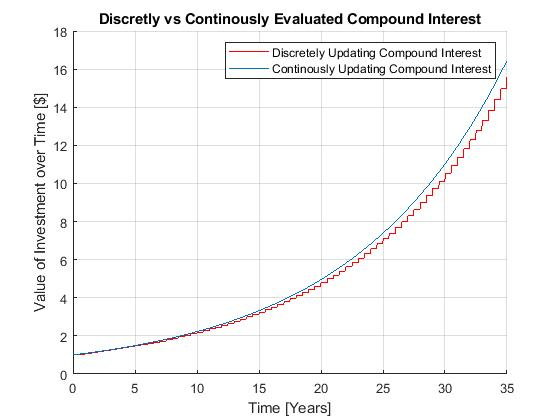
\includegraphics[width=\textwidth]{graph_final_2d.jpg}
    The final values are obtained:\\
    Discretely evaluated: t  = 35 y, final value = \$ 15.57\\
    Continuously evaluated: t = 35 y, final value = \$ 16.44
    
    \section*{$\frac{1}{2}$ Page Critique of Computer Aided Problem Solving}

    - Computers can take some input and generate an output
    - With properly defined input and instructions, a computer can expedite the problem solving process, as sometimes problem solving requires one to obtain numeric values or visualizations that are otherwise extremely tedious
    
    The core functionality of a computer as a tool in problem solving is to follow a \textit{very} specific procedure to map some given input to some output. This essentially describes the process of computation, and it is worth noting that the inputs and outputs could be in entirely different modes - numerical, visual, auditory, physical, etc. The process of problem solving, particularly regarding the empirical sciences, may involve such a mapping as a step or as a way to obtain a final solution, and for this reason computers can be particularly helpful, though one should observe that with regards to less rigorous domains of study computation may be wholly unnecessary. Additionally, though the modes of data may vary, they must be reducable to numeric (computer-readable) formats - audio may be transformed via the FFT algorithm, visuals displayed via pixel matrices and other such concepts but things like ethics are harder to condense into numeric format (though not impossible, and that answers an entirely different question). \\Computers may be thus used in creating mappings in cases where manual computation is tedious, and create immeasurable benefit in problem solving due to their higher precision and staggering (many orders of magnitude more operations per second) speed improvements over even the most technically skilled human operators. Some examples are computation of trigonometric values, logarithms, and 3D visualization, which all are possible by hand (eg. lookup table requiring incredibly large amounts of time and resources to compute, slide rule and a lot of drafting tools respectively), which computers can solve with speeds that are many orders of magnitude faster than humans.\\However, though computers have the potential to massively expedite the problem solving process, they are still vulnerable to a number of failure modes. Even if the input fed into a computer program is perfect, the mapping must be created by a human operator (assuming it's not written by a self-programming program which is again the subject of another very interesting but irrelevant paper) and the creation of this mapping from input to output is prone to all sorts of human error, and requires very precise understanding of the problem and a deep understanding of how exactly to map the input to the output. Even with all the computing resources in the world, I would be unable to solve a difficult electromechanics problem even if I had all the necessary inputs, because I wouldn't understand it and I couldn't tell a computer how to solve it for me. Not understanding the problem enough to encode it in a way that is understandable by a computer (also requiring programming knowledge) renders a computer about as useful as a paperweight for problem solving. Additional vulnerabilities are data corruption, radiation damage (rare, but can flip bits and destroy/alter output) and the quirks of various programming languages (see Javascript Equality Memes for reference), among others.\\ In conclusion, computers can vastly expedite the problem solving process for tedious, complex or repetitive tasks in systems that are numerically operationalizable (also, maybe deterministic) but are vulnerable to a host of errors and require a deep initial understanding of the problem to be able to use them and some technical skill as well. They are not an all purpose problem solving machine (yet) but rather are valuable tools that can immeasurably speed up and refine the problem solving process in the hands of a skilled operator. 

\end{document}
